\documentclass{standalone}

\usepackage{tikz}
\usetikzlibrary{math}

\begin{document}
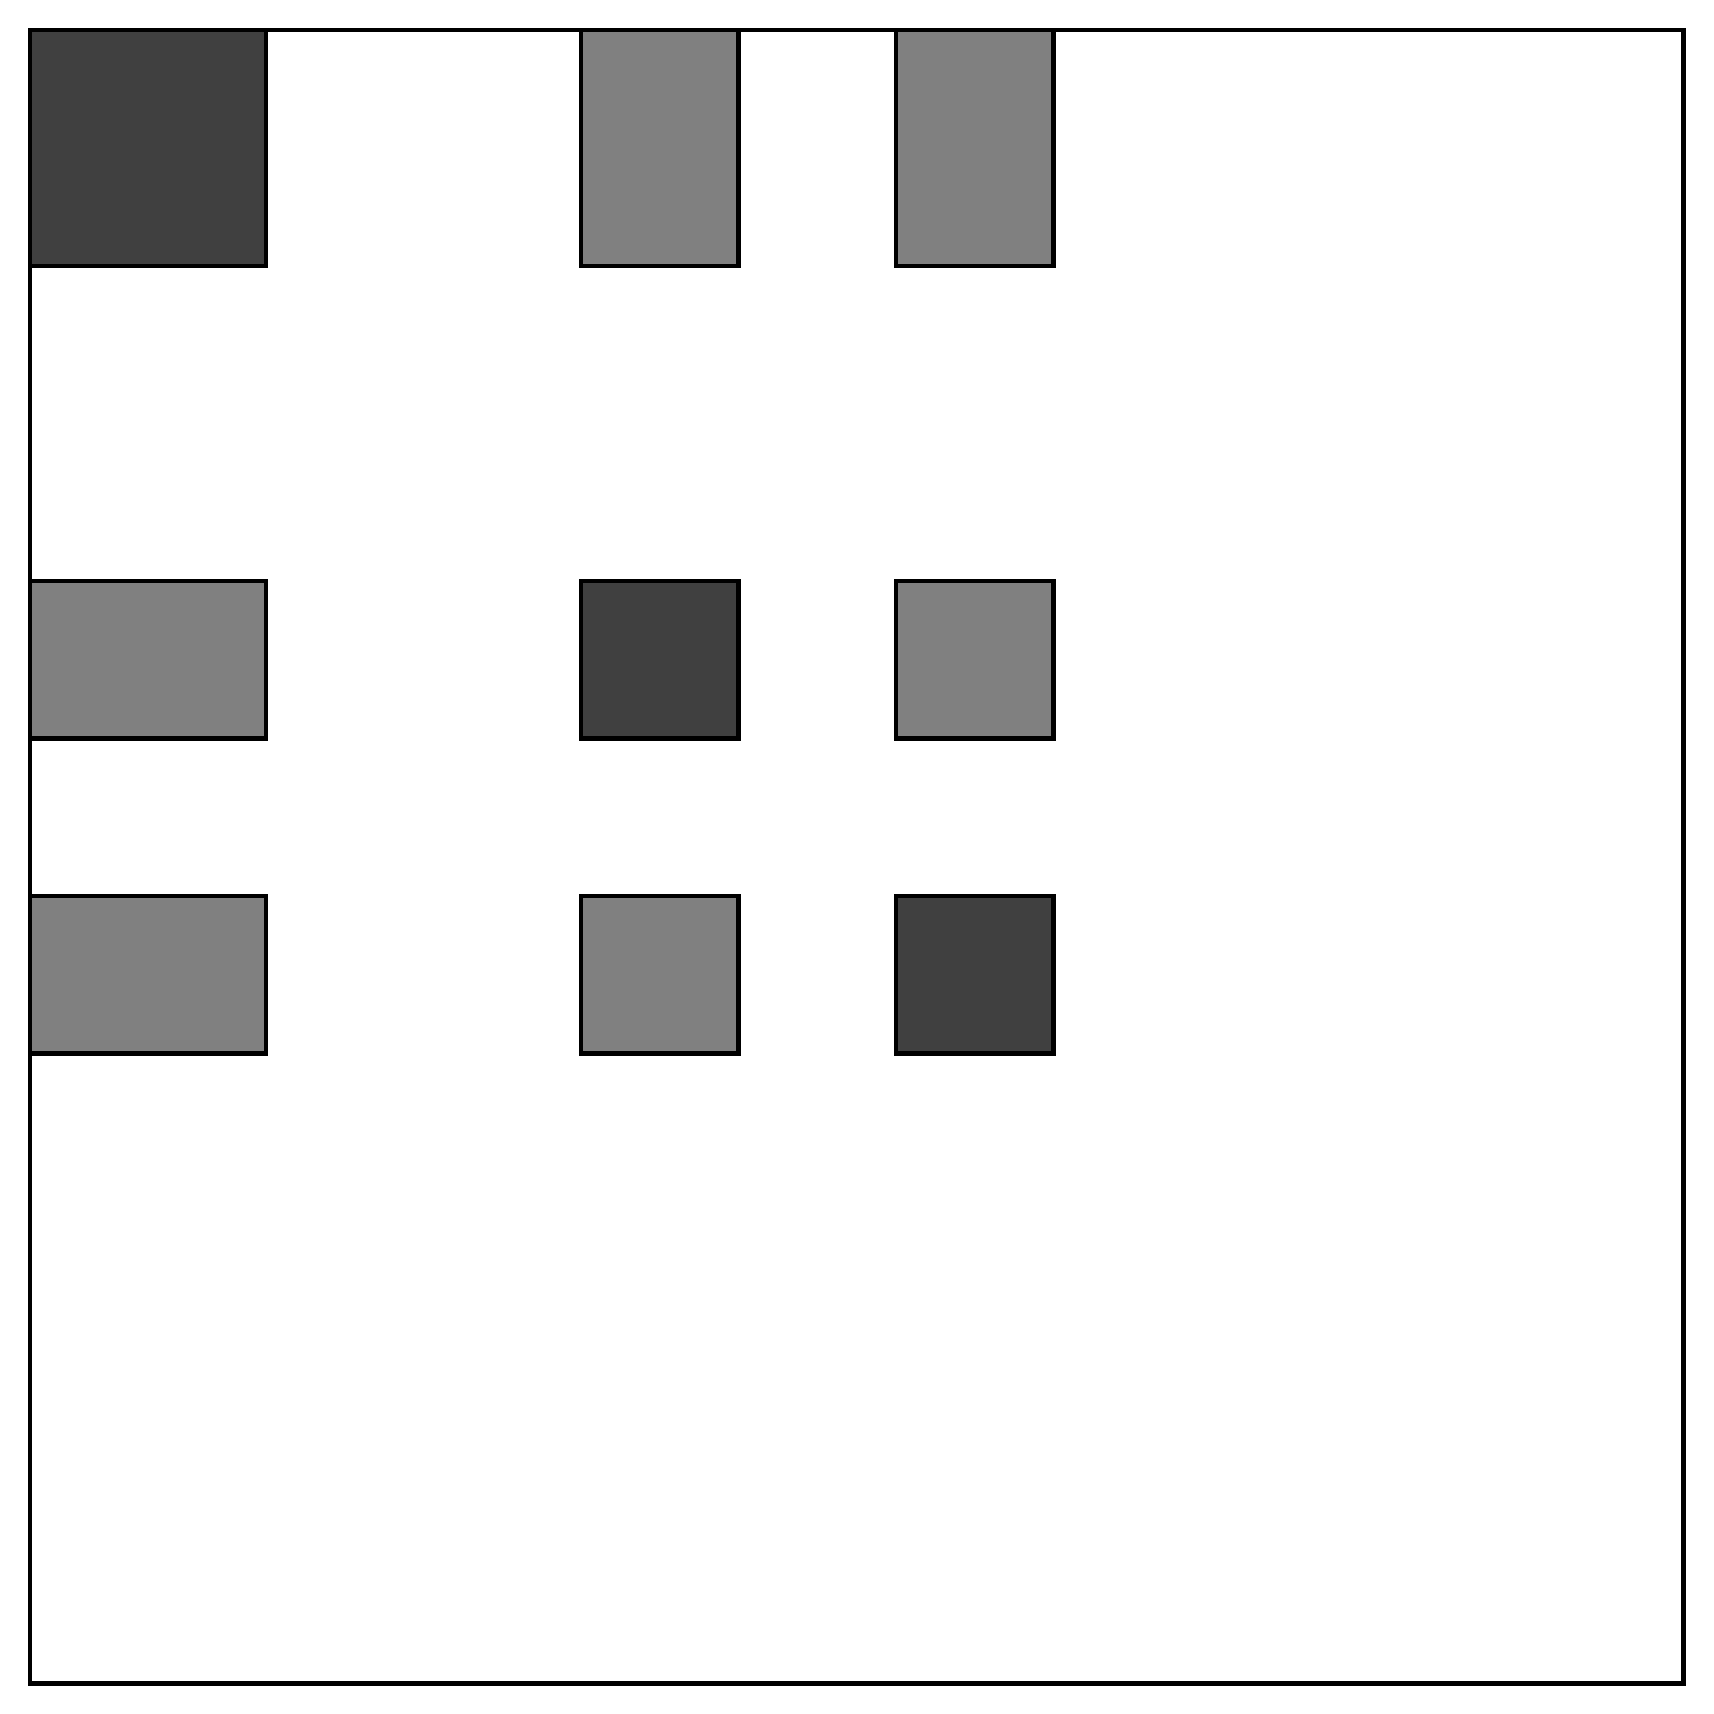
\begin{tikzpicture}
  \tikzmath{\m = 21;}
  \tikzmath{\i = 2;}
  \tikzmath{\j = 4;}

  \draw[ultra thick] (0, 0) rectangle ++(\m, \m);

  % \draw[ultra thick, fill=] (,) rectangle ++(,);
  % robot auto cov
  \draw[ultra thick, fill=darkgray] (0, \m-3) rectangle ++(3,3);
  
  % ith landmark auto cov
  \draw[ultra thick, fill=darkgray] (3+2*\i, \m-3-2*\i-2) rectangle ++(2,2);

  % jth landmark auto cov
  \draw[ultra thick, fill=darkgray] (3+2*\j, \m-3-2*\j-2) rectangle ++(2,2);

  % robot cross cov ith landmark
  \draw[ultra thick, fill=gray] (3+2*\i, \m-3) rectangle ++(2, 3);
  \draw[ultra thick, fill=gray] (0, \m-3-2*\i-2) rectangle ++(3, 2);

  % robot cross cov jth landmark
  \draw[ultra thick, fill=gray] (3+2*\j, \m-3) rectangle ++(2, 3);
  \draw[ultra thick, fill=gray] (0, \m-3-2*\j-2) rectangle ++(3, 2);

  % landmarks cross cov
  \draw[ultra thick, fill=gray] (3+2*\i, \m-3-2*\j-2) rectangle ++(2,2);
  \draw[ultra thick, fill=gray] (3+2*\j, \m-3-2*\i-2) rectangle ++(2,2);
\end{tikzpicture}
\end{document}